% Created by tikzDevice version 0.12.3 on 2020-05-24 11:17:50
% !TEX encoding = UTF-8 Unicode
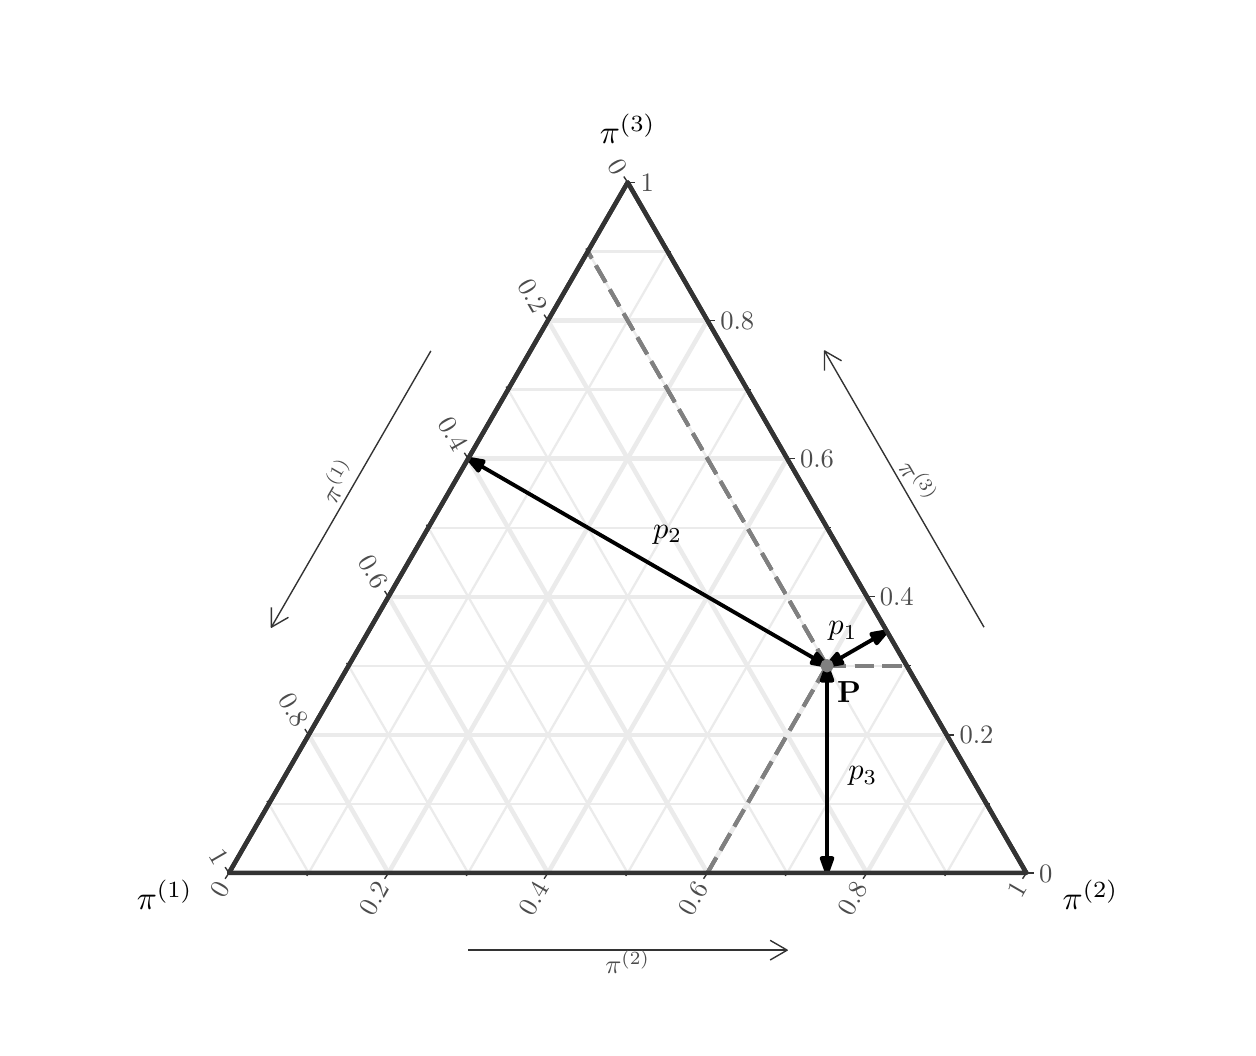
\begin{tikzpicture}[x=1pt,y=1pt]
\definecolor{fillColor}{RGB}{255,255,255}
\path[use as bounding box,fill=fillColor,fill opacity=0.00] (0,0) rectangle (433.62,361.35);
\begin{scope}
\path[clip] (  9.11,  0.00) rectangle (424.51,361.35);
\definecolor{drawColor}{RGB}{255,255,255}
\definecolor{fillColor}{RGB}{255,255,255}

\path[draw=drawColor,line width= 1.6pt,line join=round,line cap=round,fill=fillColor] (  9.11,  0.00) rectangle (424.51,361.35);
\end{scope}
\begin{scope}
\path[clip] ( 15.11,  6.00) rectangle (418.51,355.35);
\definecolor{fillColor}{RGB}{255,255,255}

\path[fill=fillColor] (216.81,305.44) --
	( 72.74, 55.91) --
	(360.88, 55.91) --
	cycle;
\definecolor{drawColor}{gray}{0.92}

\path[draw=drawColor,line width= 0.8pt,line join=round] (346.47, 80.86) -- ( 87.15, 80.86);

\path[draw=drawColor,line width= 0.8pt,line join=round] (317.66,130.77) -- (115.96,130.77);

\path[draw=drawColor,line width= 0.8pt,line join=round] (288.84,180.67) -- (144.78,180.67);

\path[draw=drawColor,line width= 0.8pt,line join=round] (260.03,230.58) -- (173.59,230.58);

\path[draw=drawColor,line width= 0.8pt,line join=round] (231.22,280.49) -- (202.40,280.49);

\path[draw=drawColor,line width= 0.8pt,line join=round] (202.40,280.49) -- (332.07, 55.91);

\path[draw=drawColor,line width= 0.8pt,line join=round] (173.59,230.58) -- (274.44, 55.91);

\path[draw=drawColor,line width= 0.8pt,line join=round] (144.78,180.67) -- (216.81, 55.91);

\path[draw=drawColor,line width= 0.8pt,line join=round] (115.96,130.77) -- (159.18, 55.91);

\path[draw=drawColor,line width= 0.8pt,line join=round] ( 87.15, 80.86) -- (101.55, 55.91);

\path[draw=drawColor,line width= 0.8pt,line join=round] (101.55, 55.91) -- (231.22,280.49);

\path[draw=drawColor,line width= 0.8pt,line join=round] (159.18, 55.91) -- (260.03,230.58);

\path[draw=drawColor,line width= 0.8pt,line join=round] (216.81, 55.91) -- (288.84,180.67);

\path[draw=drawColor,line width= 0.8pt,line join=round] (274.44, 55.91) -- (317.66,130.77);

\path[draw=drawColor,line width= 0.8pt,line join=round] (332.07, 55.91) -- (346.47, 80.86);

\path[draw=drawColor,line width= 1.6pt,line join=round] (360.88, 55.91) -- ( 72.74, 55.91);

\path[draw=drawColor,line width= 1.6pt,line join=round] (332.07,105.81) -- (101.55,105.81);

\path[draw=drawColor,line width= 1.6pt,line join=round] (303.25,155.72) -- (130.37,155.72);

\path[draw=drawColor,line width= 1.6pt,line join=round] (274.44,205.63) -- (159.18,205.63);

\path[draw=drawColor,line width= 1.6pt,line join=round] (245.62,255.54) -- (188.00,255.54);

\path[draw=drawColor,line width= 1.6pt,line join=round] (216.81,305.44) -- (216.81,305.44);

\path[draw=drawColor,line width= 1.6pt,line join=round] (216.81,305.44) -- (360.88, 55.91);

\path[draw=drawColor,line width= 1.6pt,line join=round] (188.00,255.54) -- (303.25, 55.91);

\path[draw=drawColor,line width= 1.6pt,line join=round] (159.18,205.63) -- (245.62, 55.91);

\path[draw=drawColor,line width= 1.6pt,line join=round] (130.37,155.72) -- (188.00, 55.91);

\path[draw=drawColor,line width= 1.6pt,line join=round] (101.55,105.81) -- (130.37, 55.91);

\path[draw=drawColor,line width= 1.6pt,line join=round] ( 72.74, 55.91) -- ( 72.74, 55.91);

\path[draw=drawColor,line width= 1.6pt,line join=round] ( 72.74, 55.91) -- (216.81,305.44);

\path[draw=drawColor,line width= 1.6pt,line join=round] (130.37, 55.91) -- (245.62,255.54);

\path[draw=drawColor,line width= 1.6pt,line join=round] (188.00, 55.91) -- (274.44,205.63);

\path[draw=drawColor,line width= 1.6pt,line join=round] (245.62, 55.91) -- (303.25,155.72);

\path[draw=drawColor,line width= 1.6pt,line join=round] (303.25, 55.91) -- (332.07,105.81);

\path[draw=drawColor,line width= 1.6pt,line join=round] (360.88, 55.91) -- (360.88, 55.91);
\definecolor{drawColor}{gray}{0.50}

\path[draw=drawColor,line width= 1.4pt,dash pattern=on 7pt off 3pt ,line join=round] (288.84,130.77) -- (317.66,130.77);

\path[draw=drawColor,line width= 1.4pt,dash pattern=on 7pt off 3pt ,line join=round] (288.84,130.77) -- (202.40,280.49);

\path[draw=drawColor,line width= 1.4pt,dash pattern=on 7pt off 3pt ,line join=round] (288.84,130.77) -- (245.62, 55.91);

\path[draw=drawColor,line width= 1.4pt,dash pattern=on 7pt off 3pt ,line join=round] (288.84,130.77) -- (317.66,130.77);

\path[draw=drawColor,line width= 1.4pt,dash pattern=on 7pt off 3pt ,line join=round] (288.84,130.77) -- (202.40,280.49);

\path[draw=drawColor,line width= 1.4pt,dash pattern=on 7pt off 3pt ,line join=round] (288.84,130.77) -- (245.62, 55.91);

\path[draw=drawColor,line width= 1.4pt,dash pattern=on 7pt off 3pt ,line join=round] (288.84,130.77) -- (317.66,130.77);

\path[draw=drawColor,line width= 1.4pt,dash pattern=on 7pt off 3pt ,line join=round] (288.84,130.77) -- (202.40,280.49);

\path[draw=drawColor,line width= 1.4pt,dash pattern=on 7pt off 3pt ,line join=round] (288.84,130.77) -- (245.62, 55.91);
\definecolor{drawColor}{RGB}{0,0,0}

\path[draw=drawColor,line width= 1.4pt,line join=round] (310.46,143.24) -- (288.84,130.77);
\definecolor{fillColor}{RGB}{0,0,0}

\path[draw=drawColor,line width= 1.4pt,line join=round,fill=fillColor] (306.80,138.89) --
	(310.46,143.24) --
	(304.85,142.26) --
	cycle;

\path[draw=drawColor,line width= 1.4pt,line join=round,fill=fillColor] (292.50,135.13) --
	(288.84,130.77) --
	(294.45,131.76) --
	cycle;

\path[draw=drawColor,line width= 1.4pt,line join=round] (288.84, 55.91) -- (288.84,130.77);

\path[draw=drawColor,line width= 1.4pt,line join=round,fill=fillColor] (286.90, 61.25) --
	(288.84, 55.91) --
	(290.79, 61.25) --
	cycle;

\path[draw=drawColor,line width= 1.4pt,line join=round,fill=fillColor] (290.79,125.42) --
	(288.84,130.77) --
	(286.90,125.42) --
	cycle;

\path[draw=drawColor,line width= 1.4pt,line join=round] (159.18,205.63) -- (288.84,130.77);

\path[draw=drawColor,line width= 1.4pt,line join=round,fill=fillColor] (164.79,204.64) --
	(159.18,205.63) --
	(162.84,201.27) --
	cycle;

\path[draw=drawColor,line width= 1.4pt,line join=round,fill=fillColor] (283.24,131.76) --
	(288.84,130.77) --
	(285.19,135.13) --
	cycle;
\definecolor{drawColor}{gray}{0.50}
\definecolor{fillColor}{gray}{0.50}

\path[draw=drawColor,line width= 0.9pt,line join=round,line cap=round,fill=fillColor] (288.84,130.77) circle (  1.96);
\definecolor{drawColor}{RGB}{0,0,0}

\node[text=drawColor,anchor=base,inner sep=0pt, outer sep=0pt, scale=  1.10] at (294.61,141.94) {$p_1$};

\node[text=drawColor,anchor=base,inner sep=0pt, outer sep=0pt, scale=  1.10] at (301.81, 89.54) {$p_3$};

\node[text=drawColor,anchor=base,inner sep=0pt, outer sep=0pt, scale=  1.10] at (231.22,176.87) {$p_2$};

\node[text=drawColor,anchor=base,inner sep=0pt, outer sep=0pt, scale=  1.10] at (296.85,117.64) {\textbf{P}};
\definecolor{fillColor}{RGB}{255,255,255}

\path[fill=fillColor] ( 15.11,  6.00) --
	( 15.11,355.35) --
	(216.81,355.35) --
	(216.81,305.44) --
	( 72.74, 55.91) --
	(360.88, 55.91) --
	(216.81,305.44) --
	(216.81,355.35) --
	(418.51,355.35) --
	(418.51,  6.00) --
	( 15.11,  6.00) --
	cycle;
\end{scope}
\begin{scope}
\path[clip] ( 15.11,  6.00) rectangle (418.51,355.35);

\path[] ( 15.11,  6.00) --
	( 15.11,355.35) --
	(418.51,355.35) --
	(418.51,  6.00) --
	( 15.11,  6.00) --
	( 15.11,  6.00);
\end{scope}
\begin{scope}
\path[clip] ( 15.11,  6.00) rectangle (418.51,355.35);
\definecolor{drawColor}{gray}{0.20}

\path[draw=drawColor,line width= 0.5pt,line join=round] (360.88, 55.91) -- (363.67, 55.91);

\path[draw=drawColor,line width= 0.5pt,line join=round] (332.07,105.81) -- (334.86,105.81);

\path[draw=drawColor,line width= 0.5pt,line join=round] (303.25,155.72) -- (306.04,155.72);

\path[draw=drawColor,line width= 0.5pt,line join=round] (274.44,205.63) -- (277.23,205.63);

\path[draw=drawColor,line width= 0.5pt,line join=round] (245.62,255.54) -- (248.41,255.54);

\path[draw=drawColor,line width= 0.5pt,line join=round] (216.81,305.44) -- (219.60,305.44);

\path[draw=drawColor,line width= 0.5pt,line join=round] (346.47, 80.86) -- (347.87, 80.86);

\path[draw=drawColor,line width= 0.5pt,line join=round] (317.66,130.77) -- (319.05,130.77);

\path[draw=drawColor,line width= 0.5pt,line join=round] (288.84,180.67) -- (290.24,180.67);

\path[draw=drawColor,line width= 0.5pt,line join=round] (260.03,230.58) -- (261.43,230.58);

\path[draw=drawColor,line width= 0.5pt,line join=round] (231.22,280.49) -- (232.61,280.49);

\path[draw=drawColor,line width= 0.5pt,line join=round] (216.81,305.44) -- (215.41,307.54);

\path[draw=drawColor,line width= 0.5pt,line join=round] (188.00,255.54) -- (186.60,257.63);

\path[draw=drawColor,line width= 0.5pt,line join=round] (159.18,205.63) -- (157.79,207.72);

\path[draw=drawColor,line width= 0.5pt,line join=round] (130.37,155.72) -- (128.97,157.81);

\path[draw=drawColor,line width= 0.5pt,line join=round] (101.55,105.81) -- (100.16,107.91);

\path[draw=drawColor,line width= 0.5pt,line join=round] ( 72.74, 55.91) -- ( 71.35, 58.00);

\path[draw=drawColor,line width= 0.5pt,line join=round] (202.40,280.49) -- (201.71,281.54);

\path[draw=drawColor,line width= 0.5pt,line join=round] (173.59,230.58) -- (172.89,231.63);

\path[draw=drawColor,line width= 0.5pt,line join=round] (144.78,180.67) -- (144.08,181.72);

\path[draw=drawColor,line width= 0.5pt,line join=round] (115.96,130.77) -- (115.26,131.81);

\path[draw=drawColor,line width= 0.5pt,line join=round] ( 87.15, 80.86) -- ( 86.45, 81.91);

\path[draw=drawColor,line width= 0.5pt,line join=round] ( 72.74, 55.91) -- ( 71.35, 53.81);

\path[draw=drawColor,line width= 0.5pt,line join=round] (130.37, 55.91) -- (128.97, 53.81);

\path[draw=drawColor,line width= 0.5pt,line join=round] (188.00, 55.91) -- (186.60, 53.81);

\path[draw=drawColor,line width= 0.5pt,line join=round] (245.62, 55.91) -- (244.23, 53.81);

\path[draw=drawColor,line width= 0.5pt,line join=round] (303.25, 55.91) -- (301.86, 53.81);

\path[draw=drawColor,line width= 0.5pt,line join=round] (360.88, 55.91) -- (359.48, 53.81);

\path[draw=drawColor,line width= 0.5pt,line join=round] (101.55, 55.91) -- (100.86, 54.86);

\path[draw=drawColor,line width= 0.5pt,line join=round] (159.18, 55.91) -- (158.48, 54.86);

\path[draw=drawColor,line width= 0.5pt,line join=round] (216.81, 55.91) -- (216.11, 54.86);

\path[draw=drawColor,line width= 0.5pt,line join=round] (274.44, 55.91) -- (273.74, 54.86);

\path[draw=drawColor,line width= 0.5pt,line join=round] (332.07, 55.91) -- (331.37, 54.86);

\path[draw=drawColor,line width= 1.6pt,line join=round,line cap=round] (216.81,305.44) --
	( 72.74, 55.91) --
	(360.88, 55.91) --
	(216.81,305.44);

\path[draw=drawColor,line width= 1.6pt,line join=round] (216.81,305.44) --
	(360.88, 55.91);

\path[draw=drawColor,line width= 1.6pt,line join=round] ( 72.74, 55.91) --
	(216.81,305.44);

\path[draw=drawColor,line width= 1.6pt,line join=round] (360.88, 55.91) --
	( 72.74, 55.91);
\definecolor{drawColor}{gray}{0.30}

\node[text=drawColor,anchor=base west,inner sep=0pt, outer sep=0pt, scale=  0.96] at (365.53, 52.60) {0};

\node[text=drawColor,anchor=base west,inner sep=0pt, outer sep=0pt, scale=  0.96] at (336.72,102.51) {0.2};

\node[text=drawColor,anchor=base west,inner sep=0pt, outer sep=0pt, scale=  0.96] at (307.90,152.42) {0.4};

\node[text=drawColor,anchor=base west,inner sep=0pt, outer sep=0pt, scale=  0.96] at (279.09,202.32) {0.6};

\node[text=drawColor,anchor=base west,inner sep=0pt, outer sep=0pt, scale=  0.96] at (250.28,252.23) {0.8};

\node[text=drawColor,anchor=base west,inner sep=0pt, outer sep=0pt, scale=  0.96] at (221.46,302.14) {1};

\node[text=drawColor,rotate=-60.00,anchor=base east,inner sep=0pt, outer sep=0pt, scale=  0.96] at (211.62,307.56) {0};

\node[text=drawColor,rotate=-60.00,anchor=base east,inner sep=0pt, outer sep=0pt, scale=  0.96] at (182.81,257.65) {0.2};

\node[text=drawColor,rotate=-60.00,anchor=base east,inner sep=0pt, outer sep=0pt, scale=  0.96] at (153.99,207.74) {0.4};

\node[text=drawColor,rotate=-60.00,anchor=base east,inner sep=0pt, outer sep=0pt, scale=  0.96] at (125.18,157.84) {0.6};

\node[text=drawColor,rotate=-60.00,anchor=base east,inner sep=0pt, outer sep=0pt, scale=  0.96] at ( 96.37,107.93) {0.8};

\node[text=drawColor,rotate=-60.00,anchor=base east,inner sep=0pt, outer sep=0pt, scale=  0.96] at ( 67.55, 58.02) {1};

\node[text=drawColor,rotate= 60.00,anchor=base east,inner sep=0pt, outer sep=0pt, scale=  0.96] at ( 73.28, 50.49) {0};

\node[text=drawColor,rotate= 60.00,anchor=base east,inner sep=0pt, outer sep=0pt, scale=  0.96] at (130.91, 50.49) {0.2};

\node[text=drawColor,rotate= 60.00,anchor=base east,inner sep=0pt, outer sep=0pt, scale=  0.96] at (188.53, 50.49) {0.4};

\node[text=drawColor,rotate= 60.00,anchor=base east,inner sep=0pt, outer sep=0pt, scale=  0.96] at (246.16, 50.49) {0.6};

\node[text=drawColor,rotate= 60.00,anchor=base east,inner sep=0pt, outer sep=0pt, scale=  0.96] at (303.79, 50.49) {0.8};

\node[text=drawColor,rotate= 60.00,anchor=base east,inner sep=0pt, outer sep=0pt, scale=  0.96] at (361.42, 50.49) {1};
\definecolor{drawColor}{gray}{0.20}

\path[draw=drawColor,line width= 0.5pt,line join=round] (345.56,144.72) -- (287.93,244.53);

\path[draw=drawColor,line width= 0.5pt,line join=round] (294.09,240.98) --
	(287.93,244.53) --
	(287.93,237.42);

\path[draw=drawColor,line width= 0.5pt,line join=round] (145.69,244.53) -- ( 88.06,144.72);

\path[draw=drawColor,line width= 0.5pt,line join=round] ( 88.06,151.83) --
	( 88.06,144.72) --
	( 94.22,148.27);

\path[draw=drawColor,line width= 0.5pt,line join=round] (159.18, 28.01) -- (274.44, 28.01);

\path[draw=drawColor,line width= 0.5pt,line join=round] (268.28, 24.45) --
	(274.44, 28.01) --
	(268.28, 31.56);
\definecolor{drawColor}{gray}{0.30}

\node[text=drawColor,rotate=-60.00,anchor=base,inner sep=0pt, outer sep=0pt, scale=  0.96] at (318.36,195.59) {$\pi^{(3)}$};

\node[text=drawColor,rotate= 60.00,anchor=base,inner sep=0pt, outer sep=0pt, scale=  0.96] at (115.26,195.59) {$\pi^{(1)}$};

\node[text=drawColor,anchor=base,inner sep=0pt, outer sep=0pt, scale=  0.96] at (216.81, 19.46) {$\pi^{(2)}$};
\definecolor{drawColor}{RGB}{0,0,0}

\node[text=drawColor,anchor=base,inner sep=0pt, outer sep=0pt, scale=  1.20] at (216.81,319.39) {$\pi^{(3)}$};

\node[text=drawColor,anchor=base east,inner sep=0pt, outer sep=0pt, scale=  1.20] at ( 59.61, 42.73) {$\pi^{(1)}$};

\node[text=drawColor,anchor=base west,inner sep=0pt, outer sep=0pt, scale=  1.20] at (374.01, 42.73) {$\pi^{(2)}$};
\end{scope}
\end{tikzpicture}
